\documentclass[11pt]{beamer}  %% versione proiettore
%%\documentclass[11pt,handout]{beamer} %% versione stampa
\usepackage{lucidiJb-2ed}

\mode<article>
{
  \usepackage{fullpage}
  \usepackage{hyperref}
}

\mode<presentation>
{
  \setbeamertemplate{background canvas}[vertical shading][bottom=red!10,top=blue!10]
  \usetheme{Ethereum}
  \usefonttheme[onlysmall]{structurebold}
}

\subtitle{Learning Ethereum}
\title{Introduction}
\institute{Universit\`a di Verona, Italy}
\date{January 2020}

\setbeamercovered{invisible}

\begin{document}

\begin{frame}
  \titlepage
\end{frame}

\begin{frame}
  \frametitle{What is Ethereum?}

  \begin{greenbox}{}
    An open source, globally decentralized computing infrastructure
    that executes programs called \emph{smart contracts}, written
    in a Turing-complete programming language, translated into
    bytecode and run on a virtual machine. It uses a
    blockchain to synchronize and store the system's state changes
    (key/value tuples), along
    with a cryptocurrency called \emph{ether} to meter and constrain
    execution resource costs. It enables developers to build
    decentralized applications with built-in economic functions.
  \end{greenbox}

  \begin{itemize}
  \item \emph{gas} is bought when a transaction starts, with a threshold
    gas price
  \item DApps are smart contracts + web frontend (web3)
  \end{itemize}
  
\end{frame}

\begin{frame}\frametitle{People behind Ethereum}

  \begin{center}
  \begin{tabular}{c@{\hskip 1.5cm}c}
    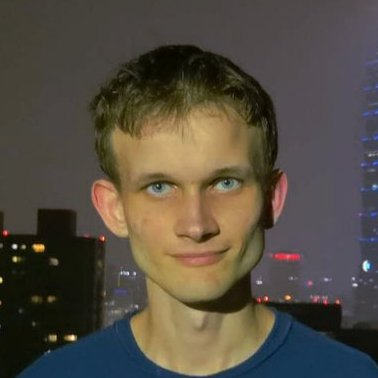
\includegraphics[scale=.3,clip=false]{pictures/vitalik_buterin.jpg} &
    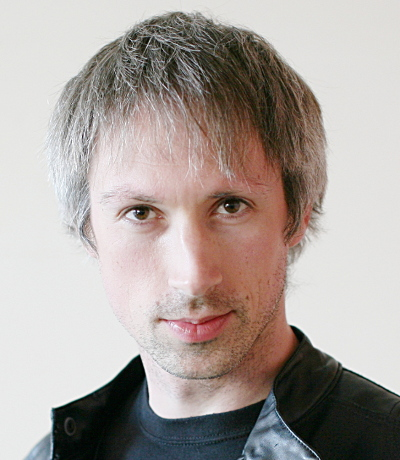
\includegraphics[scale=.247,clip=false]{pictures/gavin_wood.jpg} \\
    Vitalik Buterin & Gavin Wood
  \end{tabular}
  \end{center}
  
\end{frame}

\begin{frame}\frametitle{References used in this course}

  \begin{center}
  \begin{tabular}{c@{\hskip 1.5cm}c}
    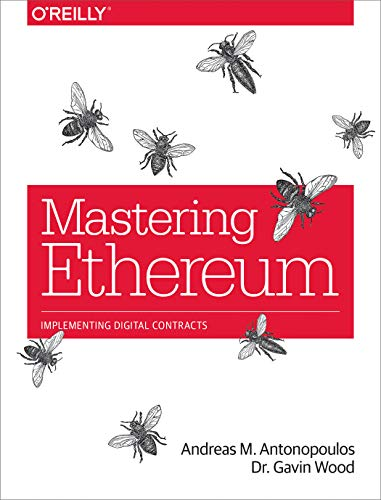
\includegraphics[scale=.3,clip=false]{pictures/mastering-ethereum.jpg} &
    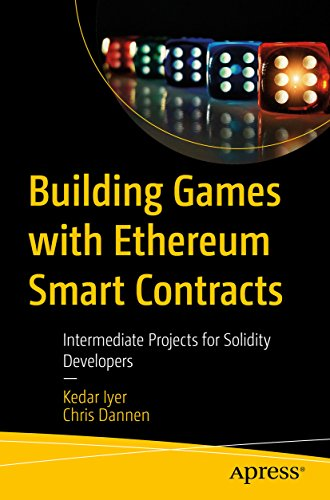
\includegraphics[scale=.3,clip=false]{pictures/building-games.jpg}
  \end{tabular}
  \end{center}

  The first: \url{https://github.com/ethereumbook/ethereumbook}

\end{frame}

\begin{frame}\frametitle{Ethereum (ETH) price over the years}

  \begin{center}
    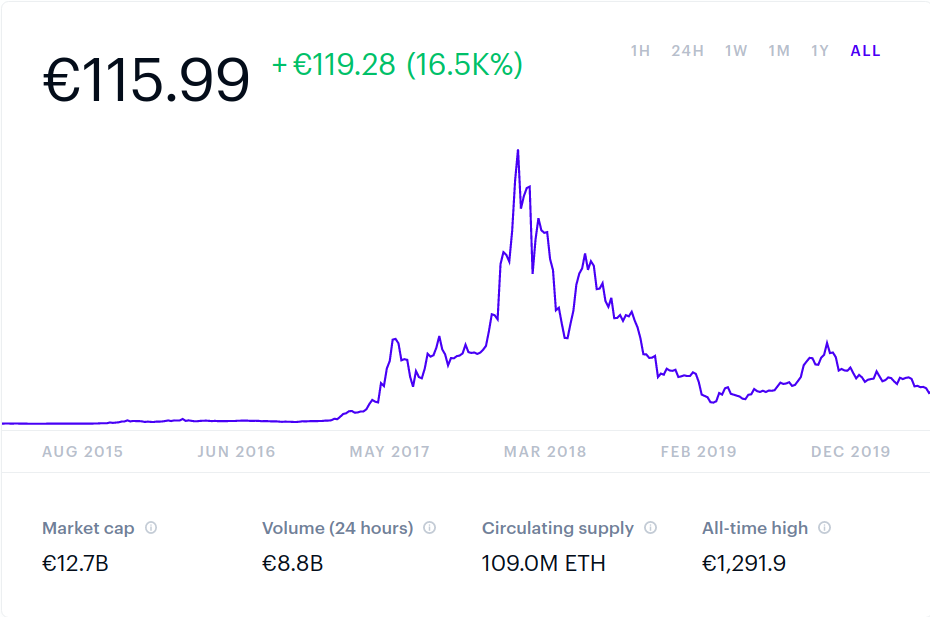
\includegraphics[scale=0.29,clip=false]{pictures/ethereum.png}
  \end{center}

\end{frame}

\begin{frame}\frametitle{Ethereum Classic (ETC) price over the years}

  \begin{center}
    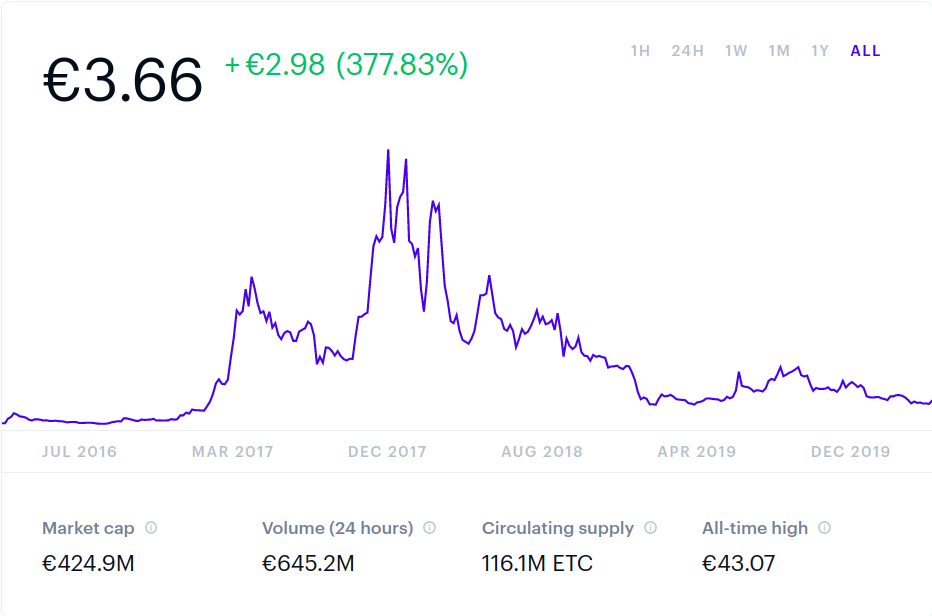
\includegraphics[scale=0.29,clip=false]{pictures/ethereum-classic.png}
  \end{center}

\end{frame}

\end{document}
